\section{Results}\label{sec:results}

\subsection{Default Placement and Batching on One Chip}\label{sec:res-default}
\begin{table*}[t]
\caption{\capTabMultichip}\label{tab:multichip}
\centering\small\setlength{\tabcolsep}{4pt}\gentable{tab_multichip}\gennote{tab_multichip}
\end{table*}

By default, AlphaFold2 inference ran on one chip of the slice. We ran the single-query script with one chip visible and
with all eight chips visible.
The steady-state call took 0.469~s with one chip visible and 0.470~s with eight. % src: results/sweep/chip_visibility_sweep.json -> [0].steady_state_seconds, [1].steady_state_seconds
With eight chips visible, chip~0 had 463~MB of HBM in use, and the other seven chips had none (Table~\ref{tab:multichip}). % src: results/sweep/chip_visibility_sweep.json -> [1].memory_stats_per_device[*].bytes_in_use, [1].memory_stats_per_device[0].device; recomputed: CV.8.hbm_in_use_bytes
The run gave no sign that the other chips took part.

Batching with \texttt{vmap} runs $B$ queries in one call on one chip. Batching did not raise throughput at any batch size
we tried.
With $B = 1$, 2, 4, and 8, the throughput was 2.051~queries/s, 1.928~queries/s, 1.487~queries/s, and 1.508~queries/s, respectively. % src: results/sweep/batching_sweep.json -> [*].batch_size, [*].throughput_proteins_per_sec
The three larger batches reached 0.94, 0.73, and 0.74 times the throughput of $B$ = 1. % src: recomputed: VM.B2.rel_B1, VM.B4.rel_B1, VM.B8.rel_B1
With $B$ = 4 and 8, one call took 38\% and 36\% longer than $B$ calls with $B$ = 1 would take. We did not study the cause. % src: recomputed: V4.vmap_B4_over_B_calls_pct, V4.vmap_B8_over_B_calls_pct; results/sweep/batching_sweep.json -> [*].batch_size
The HBM in use on chip~0 grew from 487~MB to 821~MB. The script recorded every chip, but the summary of the \texttt{vmap} runs kept chip~0 only. % src: results/sweep/batching_sweep.json -> [*].hbm_tpu0_mb; results/sweep/chip_visibility_sweep.json -> [1].memory_stats_per_device[0].device

\subsection{Multi-Query pmap and the Matched Grid}\label{sec:res-pmap}
Multi-query \texttt{pmap} runs one independent query on each chip through \texttt{jax.pmap}.
Multi-query \texttt{pmap} ran eight queries of 118 residues in parallel on all eight chips of the slice. % src: recomputed: INPUT.toy_length
Chip~0 had 644~MB of HBM in use, and the other seven chips had 445~MB to 469~MB. % src: results/sweep/sharding.json -> pmap_data_parallelism.memory_per_chip_mb; recomputed: V2.mq_mem_min, V2.mq_mem_max; results/sweep/chip_visibility_sweep.json -> [1].memory_stats_per_device[0].device
The steady-state call took 0.5435~s, and the throughput was 14.718~queries/s. % src: results/sweep/sharding.json -> pmap_data_parallelism.pmap_8chips_steady_state_seconds, pmap_data_parallelism.throughput_proteins_per_sec
Memory alone does not show how the work was divided. The division follows from \texttt{jax.pmap}, which runs one
replica per device~\cite{jaxpmap}.

\begin{figure}[t]
\centering
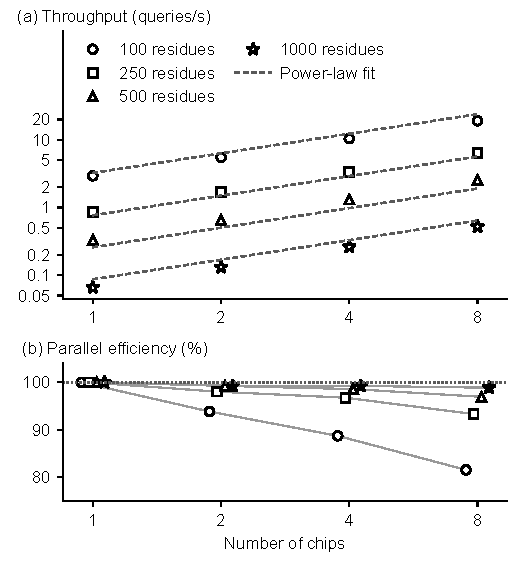
\includegraphics{figures/fig_scaling.pdf}
\caption{\capFigScaling}
\label{fig:scaling}
\end{figure}

\begin{table*}[t]
\caption{\capTabGrid}\label{tab:grid}
\centering\small\gentable{tab_grid}\gennote{tab_grid}
\end{table*}

The matched grid measures the speedup with the same script, input family, and timed region on every point.
The matched grid ran multi-query \texttt{pmap} on 1, 2, 4, and 8 chips (Fig.~\ref{fig:scaling}). The sequence lengths were 100~residues, 250~residues, 500~residues, and 1000~residues. % src: results/sweep/scaling_law_data.json -> grid[*].chips, grid[*].length
Each of the 16 points ran once. % src: results/sweep/scaling_law_data.json -> len(grid)
The Job definition committed with these results runs the 16 points in one Job, one process per point, in the order 1, 2, 4, and 8 chips, each at 100, 250, 500, and 1000 residues. % src: configs/af_spike_scaling_grid.yaml ("TOTAL=16", "for CHIPS in 1 2 4 8", "for LEN in 100 250 500 1000")
Table~\ref{tab:grid} gives the 16 throughputs. Throughput grew with the number of chips. % src: results/sweep/scaling_law_data.json -> len(grid)
At 100 residues, throughput rose from 2.935~queries/s on one chip to 19.153~queries/s on eight chips. % src: results/sweep/scaling_law_data.json -> grid[*].throughput_per_sec, grid[*].length; recomputed: SC.thr_1_L100, SC.thr_8_L100
On eight chips, the speedup was 6.53 at 100 residues, 7.47 at 250 residues, 7.76 at 500 residues, and 7.84 to 7.98 at 1000 residues. % src: recomputed: SC.speedup_8over1_L100, SC.speedup_8over1_L250, SC.speedup_8over1_L500, V4.speedup_L1000_bounds; results/sweep/scaling_law_data.json -> grid[*].length
At the same four lengths, the parallel efficiency was 81.6\%, 93.3\%, 97.0\%, and 98.0\% to 99.8\%. % src: recomputed: SC.eff_8_L100_pct, SC.eff_8_L250_pct, SC.eff_8_L500_pct, V4.eff_L1000_bounds_pct
We computed the parallel efficiency from the unrounded speedup.
At 1000 residues, the summary gives the one-chip throughput only as 0.066~queries/s, with two digits, so we give ranges at this length. % src: results/sweep/scaling_law_data.json -> grid[3].throughput_per_sec, grid[3].length

The parallel efficiency was lowest at 100 residues. To examine this difference, we compared the time of one call on
eight chips and on one chip. The call on eight chips ran eight queries, and the call on one chip ran one. We derived
the time of each call from the recorded throughput.
At 100 residues, 250 residues, and 500 residues, the call on eight chips took 0.077~s, 0.083~s, and 0.095~s longer than the call on one chip. % src: recomputed: V2.call_extra_8_L100, V2.call_extra_8_L250, V2.call_extra_8_L500; results/sweep/scaling_law_data.json -> grid[*].length
Each value comes from one run on each chip count.
At 100 residues, this extra time was 23\% of the one-chip call. % src: recomputed: V2.call_extra_8_L100_pct; results/sweep/scaling_law_data.json -> grid[0].length
At 1000 residues, the extra time lies between 0.04~s and 0.31~s. This range is too wide for a comparison with the extra time at the other lengths. % src: recomputed: V4.call_extra_8_L1000_bounds; results/sweep/scaling_law_data.json -> grid[3].length
At every call, the script passes the parameters to \texttt{jax.pmap} as an unmapped argument. The script also stacks
the inputs of all queries on chip~0 before the timer. As a result, at every call on several chips, the parameters and
the inputs of every query except the first move from chip~0 to the other chips inside the timed region. The copy of the
parameters adds time that does not depend on length, and the copy of the inputs adds time that grows with length. We
did not measure these copies. Each extra time is the difference of two single runs, so these values do not show how
the extra time depends on length. % src: src/spike_pmap_forward_pass.py ("pmapped_apply = jax.pmap(runner.apply, in_axes=(None, None, 0))", "jnp.stack(xs, axis=0)"); results/sweep/chip_visibility_sweep.json -> [1].memory_stats_per_device[0].device

A power-law fit summarizes the grid.
We fit log throughput on log chips and log length by least squares, over all 16 points. % src: results/sweep/scaling_law_data.json -> len(grid)
The fit gives a throughput of $4528 \times \mathrm{chips}^{0.9631} \times \mathrm{length}^{-1.5724}$ queries/s, with $R^2 = 0.981$ in log space. % src: results/sweep/scaling_law_data.json -> fitted_power_law; recomputed: V4.fit_printed_coeffs, SC.fit_r2
When we fit each length separately, the chip exponent ranged from 0.904 at 100 residues to 0.995 at 1000 residues. % src: recomputed: V2.chip_exp_min, V2.chip_exp_max, SC.chip_exp_L100, SC.chip_exp_L1000; results/sweep/scaling_law_data.json -> grid[*].length
The fit is descriptive, and the error of the fit changes sign with length.
The fitted value exceeds the measured throughput by up to 25.5\% at 100 residues and by up to 31.6\% at 1000 residues. % src: recomputed: V4.fit_dev_L100_pct, V4.fit_dev_L1000_pct; results/sweep/scaling_law_data.json -> grid[*].length
The fitted value falls below the measured throughput by up to 12.7\% at 250 residues and by up to 25.7\% at 500 residues. % src: recomputed: V4.fit_dev_L250_pct, V4.fit_dev_L500_pct; results/sweep/scaling_law_data.json -> grid[*].length
All four percentages are relative to the measured throughput. We do not use the fit outside the grid.

\subsection{Automatic Partitioning and External Ensemble}\label{sec:res-auto}
Automatic partitioning did not shorten the call for one query.
The two steady-state calls of this experiment took 0.472~s and 0.473~s. Single-query runs on one chip took 0.469~s to 0.471~s. % src: results/sweep/sharding.json -> mesh_auto_sharding.run_1.steady_state_seconds, mesh_auto_sharding.run_2.steady_state_seconds; recomputed: TPU.single_query_steady_min_max
Automatic partitioning runs one query inside a JAX mesh of eight chips. The axes of this mesh are marked automatic.
Our script placed no sharding annotations and did not shard the inputs.
We searched every file of AlphaFold2 at commit c77e5d2 for \texttt{jax.sharding}, \texttt{Mesh}, \texttt{PartitionSpec}, \texttt{NamedSharding}, \texttt{with\_sharding\_\allowbreak constraint}, \texttt{pjit}, \texttt{shard\_map}, and \texttt{pmap}~\cite{alphafoldrepo}. % src: git grep -nE 'jax\.sharding|\bMesh\b|PartitionSpec|NamedSharding|with_sharding_constraint|pjit|shard_map|pmap' c77e5d2 on a clone of google-deepmind/alphafold, 2026-11-23: no match in 121 files; paper-v4/SOURCE_NOTES.md section 3
None of these names occurs. The TPU Jobs did not record their AlphaFold2 commit, so the code that ran may differ from
c77e5d2.

Each of the two runs kept one value of HBM in use, 463~MB. % src: results/sweep/sharding.json -> mesh_auto_sharding.run_1.memory_per_chip_mb, mesh_auto_sharding.run_2.memory_per_chip_mb
We do not know whether this value is a mean over the chips or the value of chip~0. % src: src/spike_meshshard_forward_pass.py ("avg_hbm_per_chip_mb"); results/sweep/chip_visibility_sweep.json -> [1].memory_stats_per_device[0].device
The runs recorded neither which partitioner ran nor the placement of any array. We expect the call to run on one chip or
as a full copy on every chip. Our records cannot tell which of these two cases occurred, and we did not run a test to
find out. In both cases, no chip shares the work of another. This experiment does not test what the partitioner can do
with annotations.

AlphaFold2's own ensemble runs its members in a sequential loop (Section~\ref{sec:bg-af2}). We also built an external
ensemble. Unlike the ensemble of AlphaFold2, which combines its members inside the model, the external ensemble runs
eight full forward passes and averages one output.
We featurized one query with the eight random seeds 0 to 7. We ran one featurization per chip through \texttt{jax.pmap}. % src: recomputed: V2.ensemble_seeds; src/spike_ensemble_shard_forward_pass.py ("random_seed=i"); results/sweep/ensemble_shard.json -> num_ensemble
Then \texttt{jax.lax.pmean} averaged the logits of \texttt{predicted\_lddt} over the chips~\cite{jaxpmean}. With the
random weights of \texttt{init\_params}, these logits are zero. The global configuration of AlphaFold2 sets
\texttt{zero\_init}, so the final layer of this head starts with zero weights and biases~\cite{alphafoldrepo}. The
experiment times the collective operation and not an average of informative values.
Each of the eight chips had between 427~MB and 624~MB of HBM in use. % src: results/sweep/ensemble_shard.json -> num_chips_with_nonzero_memory, memory_stats_per_device_mb[*].bytes_in_use_mb; recomputed: V2.en_mem_min, V2.en_mem_max
The steady-state call took 0.5381~s. % src: results/sweep/ensemble_shard.json -> second_steady_state_seconds
We did not run a sequential ensemble of eight members, so we give no speedup for this experiment. The members share one
MSA and differ only by seed.
With an MSA of one sequence, the seed changes only the random masking of the MSA row. The featurization masks about 15\% of the positions of this row~\cite{alphafoldrepo}. % src: AlphaFold2 at commit c77e5d2, alphafold/model/config.py:232 ("'masked_msa_replace_fraction': 0.15", that is "15" percent), alphafold/model/tf/data_transforms.py:354-386 (make_masked_msa); paper-v4/SOURCE_NOTES.md section 3
The experiment shows that an ensemble can run on all chips of the slice. This experiment does not measure an ensemble
that a user would run for prediction.

\subsection{First Call and Compilation Cache}\label{sec:res-first}
On the TPU, the baseline run took 36.60~s for parameter initialization, 27.78~s for the first call, and 0.470~s for the steady-state call. % src: results/result_tpu-v5e-podslice.json -> init_params_seconds, first_predict_compile_and_run_seconds, second_predict_steady_state_seconds
Over the ten single-query runs of this configuration with an empty compilation cache, the first call took 27.37~s to 28.80~s. % src: recomputed: V2.tpu_first_n, TPU.single_query_first_min_max
In every August version that we have, the single-query script runs the first call with the profiler. Later versions do
so by default. The first calls of these August scripts include the profiler teardown, whose duration on the TPU was not
recorded. We cannot identify the script of the baseline run (Section~\ref{sec:platforms}). The first call of the
baseline run probably includes the profiler teardown too.
In September, the runs with the profiler measured the teardown on the T4 and on the CPU runtime. On the CPU runtime, the teardown took 31.7~s to 31.9~s. % src: recomputed: V2.sep_cpu_tail_min, V2.sep_cpu_tail_max
On the T4, the teardown took 23.7~s. % src: recomputed: SEP.gpu.0915.profiler_tail_s
The automatic-partitioning script runs no profiler. The first calls of this script took 14.76~s and 14.46~s. % src: results/sweep/sharding.json -> mesh_auto_sharding.run_1.first_predict_seconds, mesh_auto_sharding.run_2.first_predict_seconds
These calls ran inside a mesh, so we do not use them to estimate the profiler teardown.

The September runs without the profiler give first calls that exclude the teardown.
On the CPU runtime, the first call took 373.2~s to 394.7~s in the three sessions, against mean steady-state calls of 348.9~s to 359.3~s. % src: recomputed: V2.sep_cpu_first_min, V2.sep_cpu_first_max, V2.sep_cpu_steady_min, V2.sep_cpu_steady_max
On the T4, the first call took 39.59~s, against a mean steady-state call of 6.57~s. % src: recomputed: SEP.gpu.0915.first_noprofile, SEP.gpu.0915.mean

On the TPU, the compilation cache shortened parameter initialization and the first call of a second process. We ran the
baseline configuration in two processes that shared one cache directory.
Parameter initialization took 37.68~s in the first process and 5.53~s in the second. The ratio is 6.81. % src: results/sweep/compilation_cache.json -> cold.init_params_seconds, warm.init_params_seconds; recomputed: CC.speedup_init
The first call took 28.80~s in the first process and 15.19~s in the second. The ratio is 1.90. % src: results/sweep/compilation_cache.json -> cold.first_predict_seconds, warm.first_predict_seconds; recomputed: CC.speedup_first
Parameter initialization and the first call together took 66.48~s in the first process and 20.72~s in the second. % src: recomputed: CC.combined_cold, CC.combined_warm
The steady-state call took 0.470~s in the first process and 0.469~s in the second. % src: results/sweep/compilation_cache.json -> cold.steady_state_seconds, warm.steady_state_seconds
Both first calls include the profiler teardown, so we do not attribute the 15.19~s of the second process to compilation. % src: results/sweep/compilation_cache.json -> warm.first_predict_seconds
One pair of processes ran. With the trained weights, a user loads the parameters instead of calling
\texttt{init\_params}. We did not time the loading of the trained parameters.

\subsection{Single-Chip Sweeps}\label{sec:res-sweeps}
\begin{table}[t]
\caption{\capTabSweeps}\label{tab:sweeps}
\centering\small\gentable{tab_sweeps}\gennote{tab_sweeps}
\end{table}

Table~\ref{tab:sweeps} gives four sweeps on one chip, and each setting in these sweeps ran once.

Between 60 and 500 residues, the steady-state call grew from 0.208~s to 3.031~s. % src: results/sweep/sequence_length_sweep.json -> [0].num_residues, [3].num_residues, [0].steady_state_seconds, [3].steady_state_seconds
A least-squares fit of log time on log length over these four points gives a slope of 1.28. % src: recomputed: SL.exponent_k
The length exponent of the power-law fit, $-1.5724$ (Section~\ref{sec:res-pmap}), describes throughput with \texttt{apply} over 100 to 1000 residues. The slope of 1.28 describes time with \texttt{predict} over 60 to 500 residues. % src: recomputed: SL.exponent_k, SC.fit_len_exp; results/sweep/scaling_law_data.json -> grid[*].length; results/sweep/sequence_length_sweep.json -> [*].num_residues
Between neighboring lengths, the slope of log time on log length ranged from 1.33 to 2.33 on the one-chip points of the matched grid and from 0.97 to 1.44 in the sequence-length sweep. % src: recomputed: V2.local_slope_grid_1chip, V2.local_slope_sweep
No single power law fits these data closely.

The steady-state call took 0.469~s, 0.933~s, and 1.845~s with 0, 1, and 3 recycles. Each recycle added 0.459~s on average. % src: results/sweep/recycle_depth_sweep.json -> [*].steady_state_seconds, [*].num_recycle; recomputed: RD.per_recycle_s
The first call roughly doubled with one or three recycles. We did not study the cause.

The bfloat16 setting casts the parameters to bfloat16. The script does not change the activations.
The steady-state call took 0.469~s with bfloat16 parameters and 0.470~s with float32 parameters. % src: results/sweep/precision_sweep.json -> [1].steady_state_seconds, [0].steady_state_seconds
The HBM in use fell by 40.2\%, from 463~MB to 277~MB. % src: results/sweep/precision_sweep.json -> [*].hbm_bytes_in_use; recomputed: PR.d_hbm_pct
The peak memory rose by 18.5\%, from 486~MB to 576~MB. % src: results/sweep/precision_sweep.json -> [*].hbm_peak_bytes_in_use; recomputed: PR.d_peak_pct
During the cast, the chip holds both the float32 and the bfloat16 parameters, which may explain this rise. We did not
test this hypothesis. On the TPU, JAX by default computes float32 matrix products in
bfloat16~\cite{jaxmatmulprecision}. We did not change this default, which may explain why the bfloat16 parameters did
not shorten the call. We did not test this explanation.

Among the three models without templates, \texttt{model\_5} had the shortest steady-state call.
The call of \texttt{model\_5} took 0.403~s, which is 14.4\% less than the 0.471~s of \texttt{model\_3}. The call of \texttt{model\_4} took 0.472~s. % src: results/sweep/model_comparison.json -> [*].steady_state_seconds; recomputed: MC.model5_vs_model3_pct, V2.model_steady
The configurations of \texttt{model\_3} and \texttt{model\_4} set 5120 extra MSA rows, and that of \texttt{model\_5} sets 1024~\cite{alphafoldrepo}. % src: AlphaFold2 at commit c77e5d2, alphafold/model/config.py:71-81 ("'data.common.max_extra_msa': 5120"), config.py:144 ("'max_extra_msa': 1024")
The smaller number of extra MSA rows may explain the shorter call of \texttt{model\_5}. We did not test this hypothesis.
Section~\ref{sec:limitations} discusses why times differ between these sweeps and the other experiments.

\subsection{Cost at List Price}\label{sec:res-cost}
Google's on-demand price for a TPU v5e chip in us-west4 was \$1.20 per hour on November 23, 2026~\cite{googletpupricing}. % src: recomputed: V2.price_chip_hour ("read 2026-11-23")
The course provided the slice, so we did not pay this price.
At \$1.20 per chip-hour, a slice of eight chips costs \$9.60 per hour, whether one chip works or all eight do. % src: recomputed: V2.price_chip_hour, V2.price_slice_hour
On this slice, 1000 queries of 100 residues on the matched grid would cost \$0.91 with one chip working and \$0.14 with all eight. % src: recomputed: V2.cost_slice_1chip_L100, V2.cost_slice_8chip_L100 ("per 1000 queries"); results/sweep/scaling_law_data.json -> grid[*].length
At 1000 residues, 1000 queries would cost about \$40 with one chip working and \$5.11 with all eight. % src: recomputed: V2.cost_slice_1chip_L1000, V2.cost_slice_8chip_L1000 ("per 1000 queries"); results/sweep/scaling_law_data.json -> grid[*].length
TPU v5e is also offered as slices of one and four chips~\cite{googletpuv5e}.
At the same price per chip, one chip rented alone would cost \$0.11 for the 1000 queries of 100 residues, if this chip reached the throughput of one chip of our slice. % src: recomputed: V2.cost_chip_alone_L100 ("per 1000 queries"); results/sweep/scaling_law_data.json -> grid[0].length
We did not measure a chip rented alone.
At 1000 residues, the cost on a chip rented alone and the cost on the full slice differ by about 1\%. % src: recomputed: SC.cost_increase_1to8_L1000_pct, V2.cost_chip_alone_L1000; results/sweep/scaling_law_data.json -> grid[3].length
Eight chips finish the same queries sooner, but the parallel efficiency is below 100\% at every length. % src: upper limit of the parallel efficiency ("100%"); recomputed: V4.eff_L1000_bounds_pct
These costs cover steady-state calls only. They exclude parameter initialization, the first call at each new length,
featurization, and the MSA search. They also assume no recycling.
With three recycles, the steady-state call on the fixed sequence took 3.9 times as long as the call without recycling (Section~\ref{sec:res-sweeps}, Table~\ref{tab:sweeps}). % src: results/sweep/recycle_depth_sweep.json -> [*].steady_state_seconds; recomputed: V2.recycle3_over_0

\subsection{Baseline Configuration on a T4 GPU and a CPU Runtime}\label{sec:res-platforms}
Table~\ref{tab:platforms} gives the time of the steady-state call on each platform and in each session. On one TPU chip, the steady-state call took 0.470~s. % src: results/result_tpu-v5e-podslice.json -> second_predict_steady_state_seconds
On the T4, the steady-state call took 13.086~s in August and a mean of 6.57~s in September. % src: results/result_gpu-t4.json -> second_predict_steady_state_seconds; recomputed: SEP.gpu.0915.mean
On the CPU runtime, the call took 212.113~s in August and means of 348.9~s to 359.3~s in the three September sessions. % src: results/result_cpu-colab.json -> second_predict_steady_state_seconds; recomputed: V2.sep_cpu_steady_min, V2.sep_cpu_steady_max
These values come from different sessions and from different copies of the script. We measured the TPU in one period
only. The TPU results were committed between August 8 and 11, 2026. % src: recomputed: V2.first_commit, V2.ensemble_commit
The times on the T4 and on the CPU runtime changed between sessions. For these reasons, we report only the smallest
ratio over all sessions. We divided the mean steady-state call of each Colab session by the steady-state call on one
TPU chip. Each August session timed one call, so its mean is that call.
For the TPU, we used 0.471~s, the longest recorded steady-state call of the 11 single-query runs of the baseline configuration. % src: recomputed: TPU.single_query_steady_min_max, TPU.single_query_steady_n
In every session, the mean steady-state call on the T4 took more than 13.9 times as long as this call on one TPU chip. % src: recomputed: V2.min_tpu_over_t4_with_max_tpu, V4.min_tpu_over_t4_worst
On the CPU runtime, the mean steady-state call took more than 449 times as long. % src: recomputed: V4.min_tpu_over_cpu_worst
These minimum ratios use the TPU times as recorded, with three decimals. Against the 0.470~s of the baseline run on the TPU, both ratios are higher. % src: results/result_tpu-v5e-podslice.json -> second_predict_steady_state_seconds; recomputed: V2.min_tpu_over_t4_rounding_upper, V2.min_tpu_over_cpu_rounding_upper
Single calls can fall below these minimum ratios.
The fastest single call on the T4 took 6.49~s. This call lasted 13.8 times as long as the steady-state call of the baseline run on the TPU (0.470~s). % src: results/result_tpu-v5e-podslice.json -> second_predict_steady_state_seconds; recomputed: V2.t4_sep_fastest_call, V2.tpu_over_t4_fastest_call
These ratios also compare different arithmetic. On the TPU, JAX computes float32 matrix products in bfloat16 by
default~\cite{jaxmatmulprecision}.

Our records do not explain the change between sessions. Both T4 sessions report the same GPU model, driver, and
compute capability. The two T4 sessions differ at least in the copy of the script, the install commands, and the NumPy version.
NumPy was 2.5.1 in August and 2.1.3 in September. % src: recomputed: AUG.gpu.numpy, SEP.gpu.0915.numpy; git show 2755250:notebooks/alphafold_gpu_benchmark.ipynb ("jax[cuda12]"); results/repro/2026-09-15_gpu-t4/environment_gpu-t4-repro.json -> package_versions
The August sessions did not record their JAX version or their host CPU. In public clouds, instances of the same type can
differ in performance, for some providers markedly~\cite{leitner2016patterns}.
